% Preserve the official pdfLaTeX font encoding when compiling with Tectonic.
\RequirePackage[OT1]{fontenc}
\documentclass[conference,letterpaper]{IEEEtran}
\IEEEoverridecommandlockouts
\usepackage{cite}
\usepackage{amsmath,amssymb,amsfonts}
\usepackage{graphicx}
\usepackage{textcomp}
\usepackage{xcolor}
\usepackage{booktabs}
\usepackage{array}
\usepackage[hyphens]{url}

\begin{document}

\title{Feasibility Assessment of Balanced-Model Electric Vehicle Charging-Flexibility Schedules in Unbalanced Three-Phase Distribution Networks\thanks{Project Supported By Smart Grid-National Science and Technology Major Project (2025ZD0806600).}}

\author{\IEEEauthorblockN{Junxing Tan, Jun Wu, Shiting Cui, Chaofan Yang, Jiangcheng Wang}
\IEEEauthorblockA{\textit{School of Electrical and Automation Engineering}\\
\textit{Wuhan University}\\
Wuhan, China\\
2570734125@qq.com; byronwu@whu.edu.cn; 406385846@qq.com;\\
552391450@qq.com; 2383669292@qq.com}}

\maketitle

\begin{abstract}
Electric-vehicle (EV) charging schedules generated with balanced distribution-network models may violate constraints when implemented in unbalanced three-phase feeders. This paper assesses and derates precomputed vehicle-level unidirectional charging-flexibility schedules while preserving their vehicle--time allocation. A common factor scales the adjustment from a vehicle-feasible baseline to the target schedule. Nonlinear three-phase power flow checks bus voltage, voltage-unbalance factor (VUF), transformer loading, and feeder-head loading. The largest verified feasible scaling factor and the first limiting network constraint are determined at a scaling resolution of 0.002. Across 46 cases involving 15-min flexibility calls on the IEEE 13-node and European 906-bus low-voltage feeders, 32 target schedules require derating. The mean verified factors are 0.834 and 0.540, respectively; voltage magnitude or VUF is the first limiting constraint in 27 of the 32 limited cases. The results demonstrate how three-phase validation determines feasible implementation levels for balanced-model schedules and identifies the constraints governing their dispatch.
\end{abstract}

\begin{IEEEkeywords}
electric vehicles, charging flexibility, unbalanced distribution networks, three-phase power flow, feasibility assessment
\end{IEEEkeywords}

\section{Introduction}
Aggregated electric-vehicle (EV) charging provides flexibility through changes in charging power and timing. Its implementation depends on vehicle availability, power and energy requirements, and network voltage, phase-unbalance, and equipment limits. Unbalanced-network constraints have been incorporated into aggregate flexibility characterization \cite{chen2020}, coordinated charging and discharging \cite{nimalsiri2024}, and operating-envelope or aggregator-region construction \cite{russell2023,liu2024,russell2024,jalilian2026}. Data-driven approaches also reduce the computational burden of flexibility characterization \cite{wang2025}.

Three-phase network constraints can be included directly in scheduling. Churkin \emph{et al.} quantify the effects of unbalance and coordination on aggregated $P$--$Q$ flexibility using nonlinear three-phase optimal power flow (OPF) \cite{churkin2026}. Grid-aware frameworks incorporate network limits into day-ahead scheduling and real-time EV control \cite{gupta2025}, while coordinated formulations determine deliverable aggregator flexibility \cite{baharvandi2025}. However, an operator may receive a vehicle-level schedule already produced by a balanced planning model. Its feasibility must then be assessed in the detailed unbalanced feeder before dispatch.

This paper develops a pre-dispatch validation and derating procedure for balanced-model unidirectional (V1G) charging schedules. A common factor $\alpha$ scales the original vehicle--time adjustments from a feasible baseline, and nonlinear three-phase power flow identifies the largest verified feasible factor and the first limiting network constraint. A 46-case study on two benchmark feeders quantifies the retained charging-flexibility offers and reveals distinct limiting-constraint patterns.

\section{Network Feasibility Assessment}
\label{sec:method}
Consider $N$ EVs over $T=96$ fifteen-minute time slots. For EV $i$, arrival $a_i$, departure $d_i$, initial energy $E_i^0$, target energy $E_i^{\mathrm{tar}}$, charging efficiency $\eta_i^c$, and power limit are fixed inputs. Let $u_{i,t}$ be grid-side charging power and $\Delta t=0.25$ h. The baseline uniformly supplies the required energy over the availability window:
\begin{equation}
u^0_{i,t}=\frac{E_i^{\mathrm{tar}}-E_i^0}{\eta_i^c\Delta t(d_i-a_i)},\quad a_i\leq t<d_i,
\label{eq:baseline}
\end{equation}
and is zero otherwise. Vehicle feasibility and detailed-network feasibility of this baseline are prerequisites for assessment.

The balanced planning model first maximizes aggregate call-slot charging power in a linear program (LP) using vehicle-derived power bounds and finite-difference network sensitivities. Its nodal target is checked by nonlinear balanced power flow and reduced toward the baseline when needed. A trajectory LP then maximizes the achievable fraction of that nodal increment subject to availability, power, energy, and exact departure-target constraints. At the selected fraction, a reconstruction LP minimizes total absolute deviation from the baseline, with a $10^{-5}$ throughput term, to obtain the 96-slot target $u^B$. Balanced-network checks may further reduce this fraction. Discharging is fixed to zero.

The resulting vehicle-level schedule is then assessed in the detailed three-phase feeder. This assessment covers all 96 slots, including charging adjustments outside the call slot (Fig.~\ref{fig:workflow}).

\begin{figure}[t]
\centering
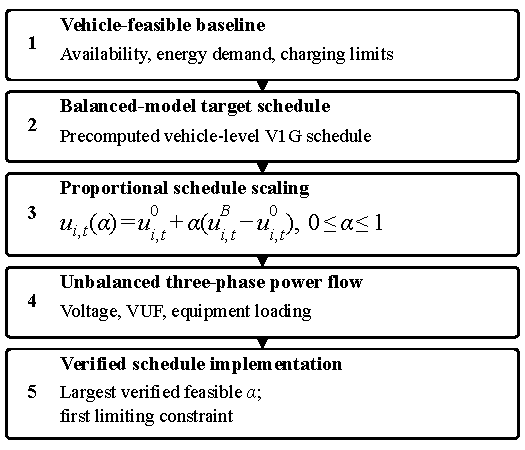
\includegraphics[width=\columnwidth]{figures/fig1_network_feasibility_workflow.pdf}
\caption{Network-feasibility assessment of a fixed charging schedule.}
\label{fig:workflow}
\end{figure}

\subsection{Proportional Scaling and Vehicle Feasibility}
The candidate charging schedule is
\begin{equation}
u_{i,t}(\alpha)=(1-\alpha)u^0_{i,t}+\alpha u^B_{i,t},\quad 0\leq\alpha\leq1.
\label{eq:scaling}
\end{equation}
Thus, $\alpha=0$ gives the baseline and $\alpha=1$ the target. Intermediate values scale the original adjustment without changing its vehicle or time allocation.

Under continuous V1G power and fixed efficiency, battery energy is affine in the charging powers. Availability, power bounds, cumulative-energy bounds, and departure equalities therefore define a convex set $\mathcal C=\{u:Au=b,\;Gu\leq h\}$. Both endpoints satisfy the same constraints, so
\begin{equation}
\begin{aligned}
Au(\alpha)&=(1-\alpha)b+\alpha b=b,\\
Gu(\alpha)&\leq(1-\alpha)h+\alpha h=h.
\end{aligned}
\label{eq:vehicleconvexity}
\end{equation}
Consequently, the interpolated schedule preserves vehicle feasibility, including $E_i(d_i)=E_i^{\mathrm{tar}}$. Discrete charging levels, minimum nonzero power, and other nonconvex charger constraints require an implementable charging allocation followed by feasibility checks.

\subsection{Three-Phase Network Checks}
Each EV remains at its assigned bus and phase in the detailed OpenDSS model \cite{opendss2020}. A schedule passes when all energized bus voltages satisfy $0.95\leq V\leq1.06$ p.u., voltage-unbalance factor (VUF) at three-phase buses is at most 2\%, and transformer and feeder-head loading are each at most 1.0 p.u. Here
\begin{equation}
\mathrm{VUF}=100\frac{|V_2|}{|V_1|},
\label{eq:vuf}
\end{equation}
where $V_1$ and $V_2$ are positive- and negative-sequence voltage magnitudes. Transformer loading uses the maximum terminal apparent power divided by its rating. Feeder-head loading uses three-phase apparent power with bases of 5 MVA for IEEE13 and 0.8 MVA for LV906.

\subsection{Scaling-Factor Determination}
The search evaluates $\alpha=0,0.02,\ldots,1$. When a violation is detected, the interval between the first infeasible coarse point and its preceding feasible point is refined with nine equally spaced interior values. Let $\alpha_L$ and $\alpha_U$ denote the adjacent feasible and infeasible samples at this transition after refinement. Their spacing satisfies
\begin{equation}
0<\alpha_U-\alpha_L\leq0.002.
\label{eq:bracket}
\end{equation}
The violated constraint at $\alpha_U$ identifies the corresponding network limitation. A feasible target at $\alpha=1$ allows full implementation.

Full-grid validation uses the grid $\mathcal G=\{0,0.002,\ldots,1\}$. Let $\mathcal F_{\mathcal G}$ contain the factors in $\mathcal G$ whose schedules satisfy the network constraints throughout all 96 slots. The \emph{largest verified feasible scaling factor} is $\max\mathcal F_{\mathcal G}$. Evaluating all 501 grid points identifies the feasible--infeasible transitions and any subsequent return to feasibility.

\section{Test Systems and Study Cases}
\label{sec:cases}
The IEEE 13-node (IEEE13) and European 906-bus low-voltage (LV906) feeders are implemented in OpenDSS \cite{dugan2009,ieeelv}. IEEE13 planning uses the positive-sequence representation. LV906 planning replaces native phase-specific loads with balanced three-phase wye loads while preserving each bus's aggregate active and reactive demand, and balances EV injections across phases. Validation restores the original feeder and EV phase assignments. Fig.~\ref{fig:feeders} shows the two test systems.

\begin{figure}[t]
\centering
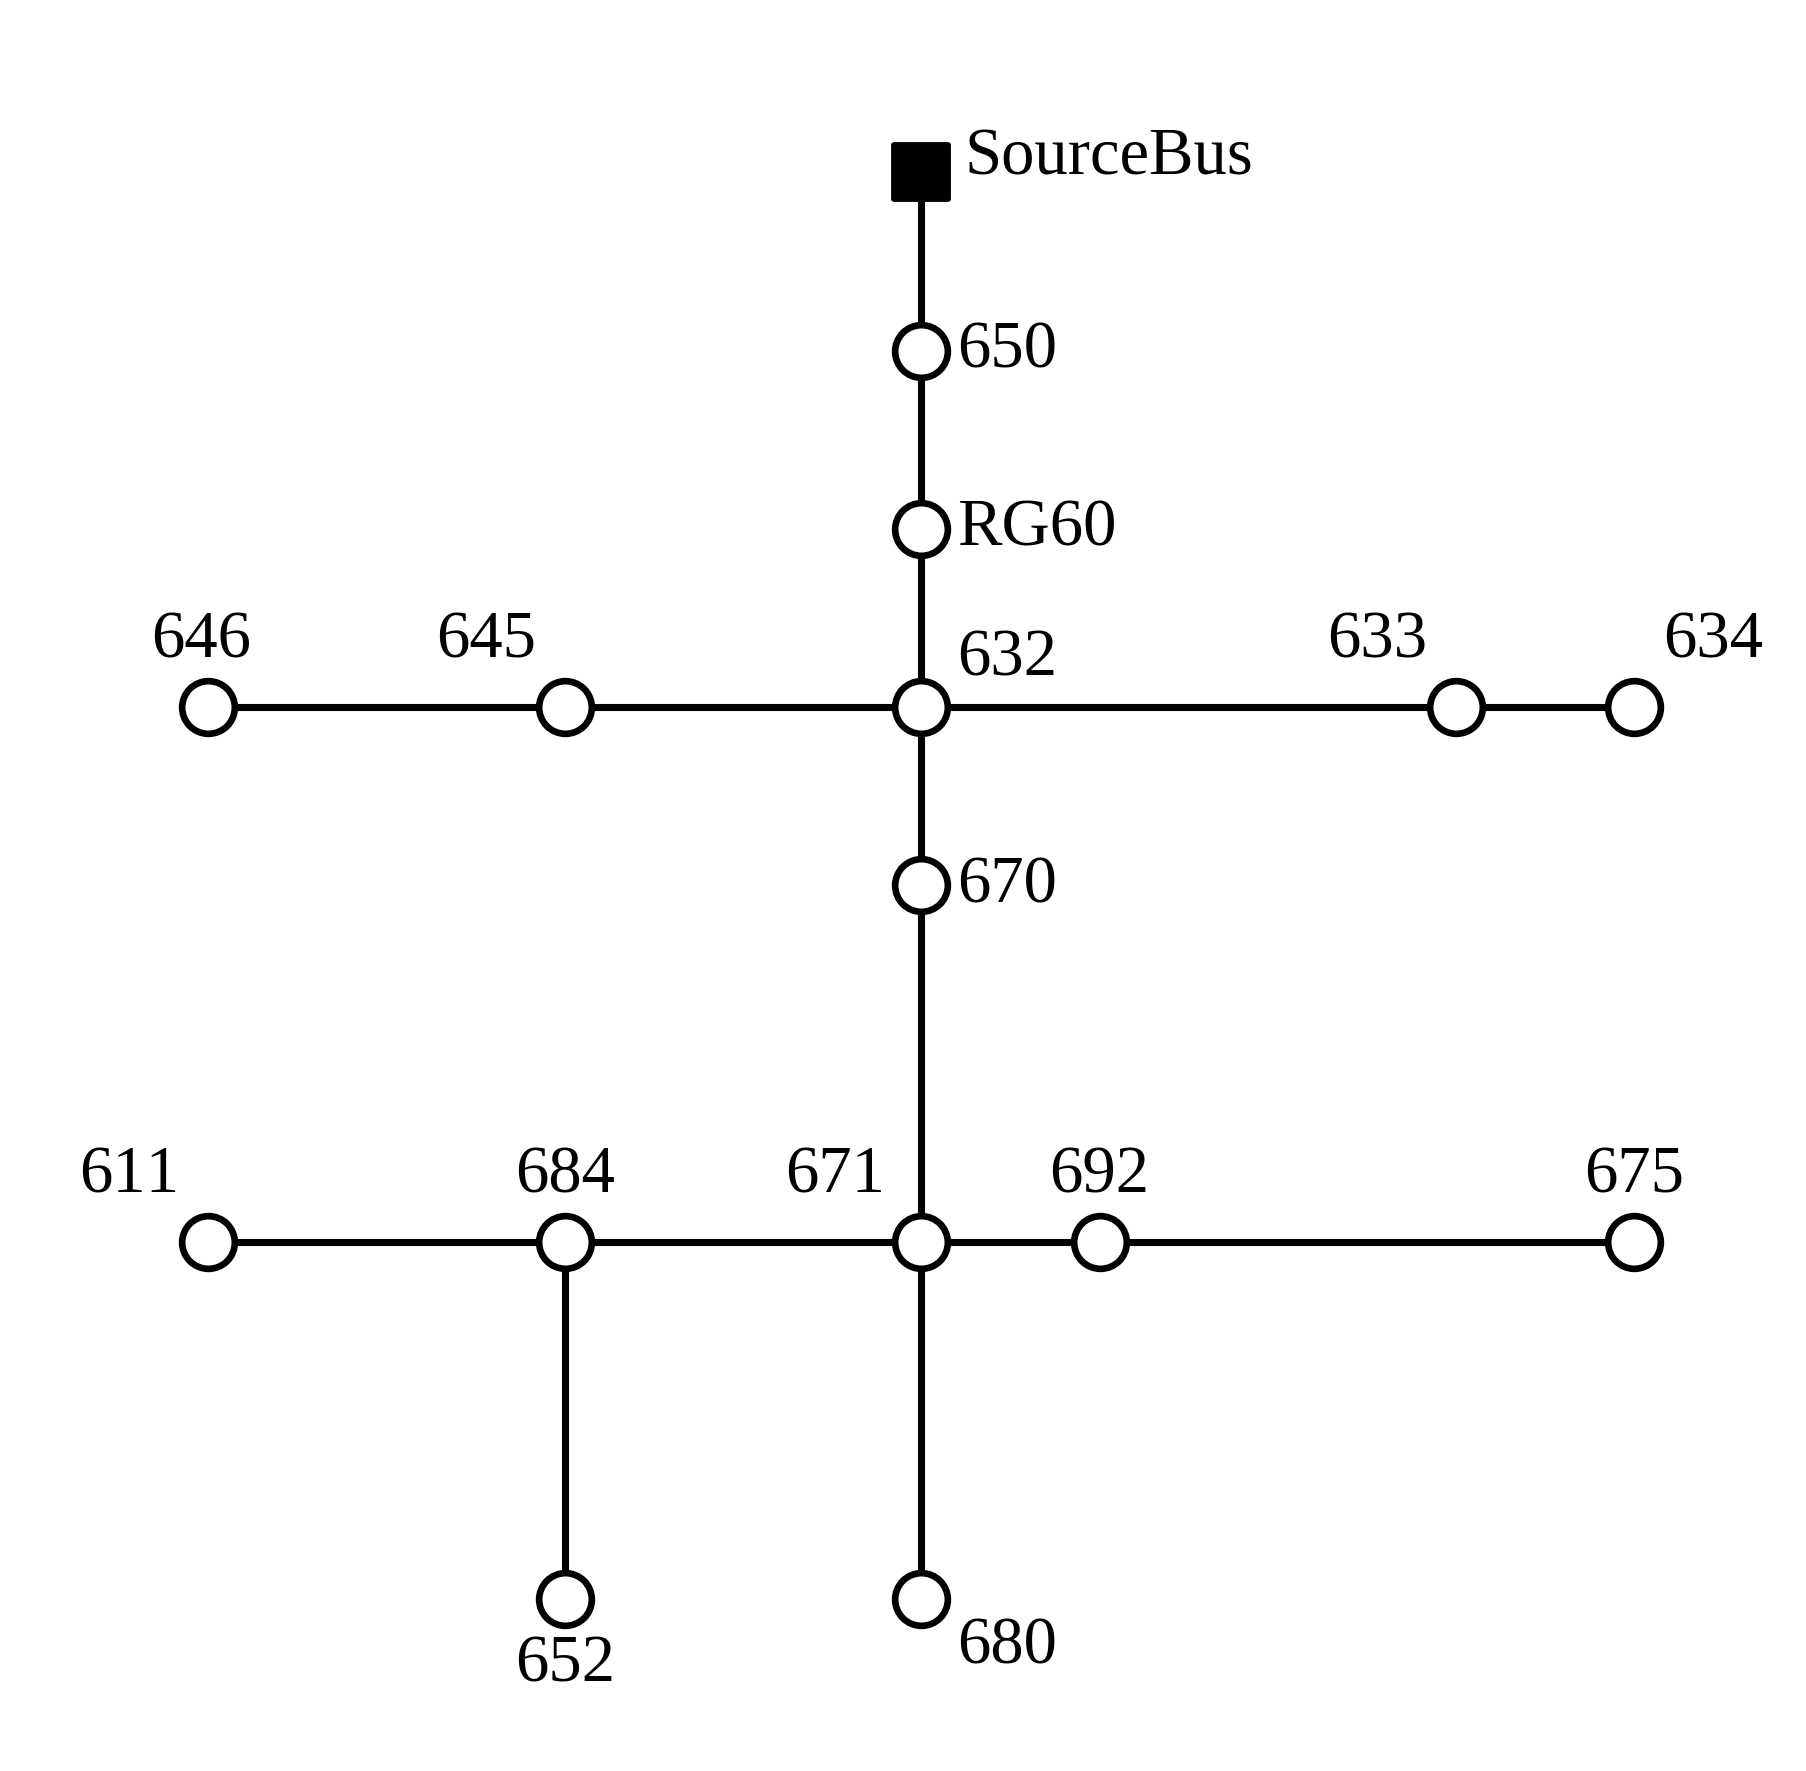
\includegraphics[width=0.82\columnwidth]{figures/fig2a_ieee13_topology.png}\par
{\footnotesize (a) IEEE 13-node feeder}\par\smallskip
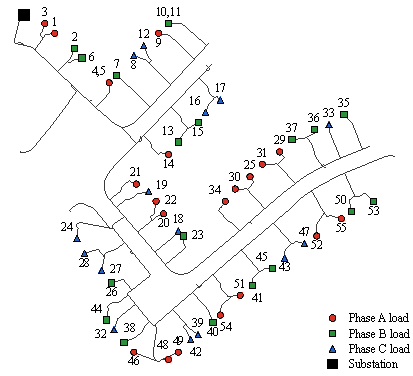
\includegraphics[width=0.82\columnwidth]{figures/fig2b_lv906_topology.pdf}\par
{\footnotesize (b) European 906-bus LV feeder}
\caption{Test distribution feeders. In (b), numbered markers identify the 55 load points; colors and shapes indicate phase assignments.}
\label{fig:feeders}
\end{figure}

EV inputs are drawn from a pool of 3,568 vehicle-day records from the 2022 National Household Travel Survey \cite{fhwa2022}. Overnight availability runs from the final home arrival to the next occurrence of that vehicle-day's first home-departure time. Only windows fully contained in the noon-to-noon horizon are retained, with endpoints rounded inward to 15-min slots. Sampling urgency is trip energy divided by the energy deliverable at 7.2 kW and efficiency 0.95 over the unrounded parking duration. For each call time, candidates must be parked, have trip energy at most 63 kWh, and have urgency in $(0,1]$. Records are sampled without replacement within a scenario, using survey weights multiplied by a Gaussian kernel of bandwidth 0.14 around a prescribed survey-weighted urgency rank.

Battery capacities are 50, 60, 70, 82, or 90 kWh, with weights 0.15, 0.25, 0.25, 0.20, and 0.15 renormalized over capacities whose 70\% usable energy covers the trip energy. Charging powers are 7.2 or 11 kW, sampled with probabilities 0.75 and 0.25. Efficiency is 0.95; target and reserve energies are 0.9 and 0.2 of capacity. Initial energy is the target minus trip energy, calculated as 0.30 kWh per reported mile.

Phase counts follow prescribed 1:1:1, 2:1:1, or 4:1:1 quotas, with shuffled vehicle assignments. Candidate connections comprise 12 single-phase wye bus--phase load points in IEEE13 and 55 in LV906. After selecting phase and near/far zone, a point is drawn in proportion to native-load kW; the far zone is the upper third by shortest-path line distance from the source.

Six EV realizations are used for each feeder--call-time pair, with calls at 00:00, 02:00, 06:00, and 19:00, giving 48 candidates. One IEEE13 baseline is network-infeasible and another case lacks a valid balanced target, leaving 22 IEEE13 and 24 LV906 cases. Table~\ref{tab:setup} gives their scale.

\begin{table}[t]
\caption{V1G Study Cases}
\label{tab:setup}
\centering
\footnotesize
\setlength{\tabcolsep}{3pt}
\begin{tabular}{lrrr}
\toprule
Feeder & Cases & EVs/case$^a$ & Scheduled offer (kW)$^a$\\
\midrule
IEEE13 & 22 & 173 [65--337] & 940 [237--1942]\\
LV906 & 24 & 29.5 [11--54] & 174 [11--261]\\
\bottomrule
\multicolumn{4}{l}{$^a$Median [minimum--maximum] across study cases.}
\end{tabular}
\end{table}

\section{Results and Discussion}
\label{sec:results}
\subsection{Schedule Feasibility}
Across the 46 cases, 32 target schedules cannot be implemented in full. Thirty have a largest verified feasible factor below 0.95 (65.2\%), and 16 fall below 0.5. The overall mean is 0.681 and the median is 0.719. Hereafter, reported $\alpha$ denotes this verified value.

For a scheduled call-slot offer $\Delta P_{\mathrm{sched}}$, the verified offer is $\Delta P_{\mathrm{feas}}=\alpha\Delta P_{\mathrm{sched}}$. Fig.~\ref{fig:offerfeasible} compares these quantities: the $y=x$ line denotes full implementation, and the vertical gap shows the reduction in the fixed target adjustment. Similar scheduled offers can yield substantially different verified offers.

\begin{figure}[t]
\centering
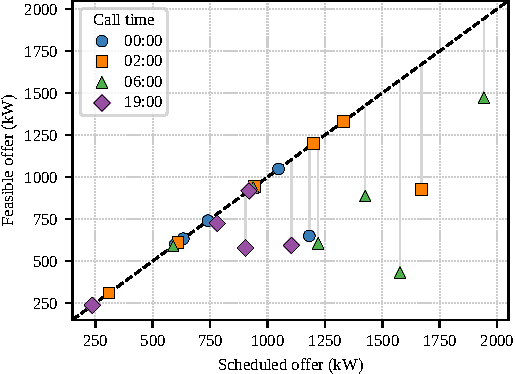
\includegraphics[width=0.92\columnwidth]{figures/fig3_ieee13_scheduled_vs_feasible_offer.pdf}\par
{\footnotesize (a) IEEE13}\par\smallskip
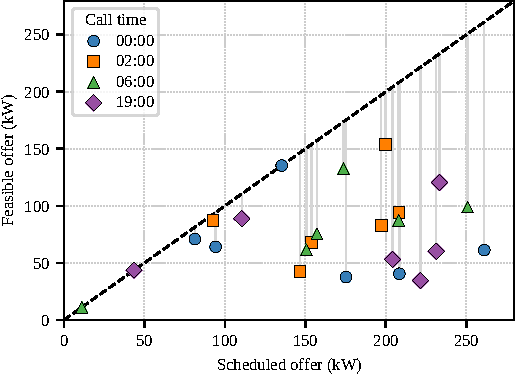
\includegraphics[width=0.92\columnwidth]{figures/fig3_lv906_scheduled_vs_feasible_offer.pdf}\par
{\footnotesize (b) LV906}
\caption{Scheduled and verified feasible EV charging-flexibility offers.}
\label{fig:offerfeasible}
\end{figure}

Table~\ref{tab:primary} and Fig.~\ref{fig:alpha} summarize the distribution. IEEE13 has a mean factor of 0.834 and a median of 0.999; 11 of 22 targets are fully implementable. LV906 has a mean of 0.540 and a median of 0.446; only 3 of 24 reach $\alpha=1$. The mean difference is 0.294, with a case-level bootstrap 95\% interval of [0.144, 0.436] for IEEE13 minus LV906. The LV906 schedules therefore undergo substantially greater derating in this case study.

\begin{table}[t]
\caption{Largest Verified Feasible Scaling Factors}
\label{tab:primary}
\centering
\footnotesize
\begin{tabular}{lrrrrr}
\toprule
Feeder & $n$ & Mean & Median & $\alpha<0.95$ & $\alpha<1$\\
\midrule
IEEE13 & 22 & 0.834 & 0.999 & 9 & 11\\
LV906 & 24 & 0.540 & 0.446 & 21 & 21\\
Overall & 46 & 0.681 & 0.719 & 30 & 32\\
\bottomrule
\end{tabular}
\end{table}

\begin{figure}[t]
\centering
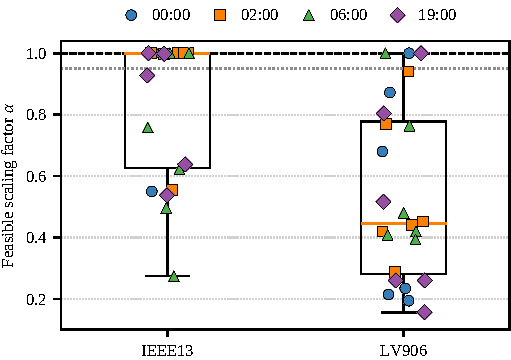
\includegraphics[width=\columnwidth]{figures/fig4_feasible_scaling_distribution.pdf}
\caption{Verified feasible scaling factors. Boxes show the interquartile range (IQR) and median; whiskers reach the extreme observations within 1.5 IQR of the box. Symbols denote cases by call time. Dashed and dotted lines mark $\alpha=1$ and $0.95$, respectively.}
\label{fig:alpha}
\end{figure}

On the 501-point grid, the feasible factors form a single consecutive sequence beginning at $\alpha=0$ in each of the 46 cases, with no infeasible-to-feasible recovery. For all 32 limited cases, the largest verified feasible factor equals $\alpha_L$ and $\alpha_U=\alpha_L+0.002$. The endpoint pairs at 19:00 for realization 28 are [0.538, 0.540] on IEEE13 and [0.156, 0.158] on LV906. The other 14 cases are feasible at $\alpha=1$.

\subsection{Limiting Network Constraints}
In all 32 limited cases, the first network violation occurs within the corresponding 15-min call. Fig.~\ref{fig:boundary} shows 20 low-voltage, two high-voltage, five VUF, and five transformer-loading cases. Voltage magnitude or VUF thus accounts for 27/32 cases (84.4\%).

Among the 11 limited IEEE13 cases, five are transformer-limited, five VUF-limited, and one low-voltage-limited. All 21 limited LV906 cases are voltage-limited: 19 by low voltage and two by high voltage. The differing patterns show why the aggregate balanced-model offer alone is insufficient to characterize implementation of its vehicle-level allocation.

\begin{figure}[t]
\centering
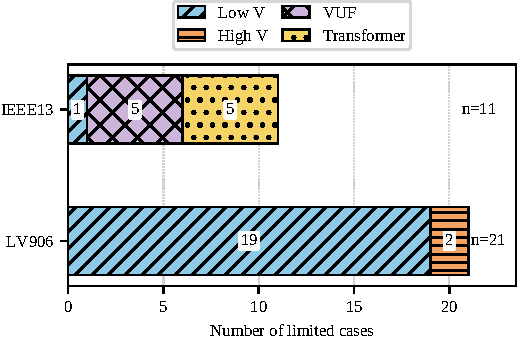
\includegraphics[width=\columnwidth]{figures/fig5_limiting_network_constraints.pdf}
\caption{First limiting network constraints at the adjacent infeasible sample.}
\label{fig:boundary}
\end{figure}

\subsection{Computational Time}
Table~\ref{tab:runtime} reports per-case runtimes for serial execution. Search-only time covers the coarse scan and local refinement. Time with preparation includes model initialization, balanced-target generation, baseline/network preparation, and the scaling-factor search. The full 501-point grid assessment takes a median of 17.64 s on IEEE13 and 1182.78 s on LV906.

\begin{table}[t]
\caption{Per-Case Computation Time in Seconds}
\label{tab:runtime}
\centering
\footnotesize
\setlength{\tabcolsep}{3pt}
\begin{tabular}{lll}
\toprule
Feeder & Search only & With preparation$^a$\\
\midrule
IEEE13 & 1.80 [1.36--3.90] & 8.76 [4.88--31.41]\\
LV906 & 119.14 [24.28--146.39] & 124.86 [29.51--153.46]\\
\bottomrule
\multicolumn{3}{l}{Entries are median [minimum--maximum].}\\
\multicolumn{3}{l}{$^a$Includes the four preparation/search stages specified in the text.}
\end{tabular}
\end{table}

\subsection{Operational Use and Extensions}
The common factor provides schedule-specific derating while retaining the original vehicle--time allocation. Network-aware redistribution across vehicles or time slots enlarges the scheduling choices and may retain more flexibility. This provides a natural extension from assessment of a given schedule to network-aware schedule optimization.

The assessment can be integrated into a day-ahead-to-real-time control chain. Before dispatch, the aggregator updates network conditions and EV states and determines the feasible scaling factor. Discrete charger powers require an energy-consistent allocation followed by vehicle and network checks. Communication delays and new arrivals require updated state estimates, operating headroom, and rolling reassessment, with each revised dispatch checked before implementation.

\section{Conclusion}
This paper assesses precomputed V1G charging-flexibility schedules through proportional scaling and nonlinear three-phase power-flow checks. The procedure quantifies the feasible implementation level of a given vehicle--time allocation and identifies the first limiting network constraint at a scaling resolution of 0.002.

Across 46 cases, 32 target schedules require derating. Mean verified factors are 0.834 for IEEE13 and 0.540 for LV906. Voltage magnitude or VUF is the first limitation in 27 of the 32 limited cases, and all 21 limited LV906 cases are voltage-limited. These results demonstrate the value of three-phase validation in determining network-feasible EV charging-flexibility offers before dispatch.

\IEEEtriggeratref{7}
\begin{thebibliography}{00}
\bibitem{chen2020} X. Chen, E. Dall'Anese, C. Zhao, and N. Li, ``Aggregate power flexibility in unbalanced distribution systems,'' \emph{IEEE Trans. Smart Grid}, vol. 11, no. 1, pp. 258--269, Jan. 2020, doi: 10.1109/TSG.2019.2920991.

\bibitem{nimalsiri2024} N. I. Nimalsiri, E. L. Ratnam, D. Smith, C. P. Mediwaththe, and S. K. Halgamuge, ``A distributed coordination approach for the charge and discharge of electric vehicles in unbalanced distribution grids,'' \emph{IEEE Trans. Ind. Informat.}, vol. 20, no. 3, pp. 3551--3562, Mar. 2024, doi: 10.1109/TII.2023.3310741.

\bibitem{russell2023} J. S. Russell, P. Scott, and J. Iria, ``Robust operating envelopes with phase unbalance constraints in unbalanced three-phase networks,'' in \emph{2023 IEEE PES Innovative Smart Grid Technologies--Asia (ISGT Asia)}, Auckland, New Zealand, 2023, pp. 1--5, doi: 10.1109/ISGTAsia54891.2023.10372617.

\bibitem{liu2024} B. Liu and J. H. Braslavsky, ``Robust dynamic operating envelopes for DER integration in unbalanced distribution networks,'' \emph{IEEE Trans. Power Syst.}, vol. 39, no. 2, pp. 3921--3936, Mar. 2024, doi: 10.1109/TPWRS.2023.3308104.

\bibitem{russell2024} J. S. Russell, P. Scott, and J. Iria, ``Network-secure aggregator operating regions with flexible dispatch envelopes in unbalanced systems,'' \emph{Electr. Power Syst. Res.}, vol. 235, Art. no. 110728, Oct. 2024, doi: 10.1016/j.epsr.2024.110728.

\bibitem{jalilian2026} A. Jalilian, D. Deka, M. U. Hashmi, and D. Van Hertem, ``Coordinated dynamic operating envelopes for unlocking additional flexibility at grid edge,'' 2026, arXiv:2604.17081. [Online]. Available: \url{https://arxiv.org/abs/2604.17081}

\bibitem{wang2025} S. Wang, L. Du, and X. Chen, ``Bayesian active learning-based soft data space calibration for system-wise aggregate flexibility characterization,'' \emph{IEEE Trans. Smart Grid}, vol. 16, no. 4, pp. 3017--3029, Jul. 2025, doi: 10.1109/TSG.2025.3555951.

\bibitem{churkin2026} A. Churkin, W. Kong, P. Mancarella, and E. A. Mart\'inez Cese\~na, ``Exposing barriers to flexibility aggregation in unbalanced distribution networks,'' Jun. 2026, arXiv:2408.06516v4. [Online]. Available: \url{https://arxiv.org/abs/2408.06516v4}

\bibitem{gupta2025} R. K. Gupta, S. A. S. Fahmy, M. Chevron, R. Vasapollo, E. Figini, and M. Paolone, ``Grid-aware scheduling and control of electric vehicle charging stations for dispatching active distribution networks: Theory and experimental validation,'' \emph{IEEE Trans. Smart Grid}, vol. 16, no. 2, pp. 1575--1589, Mar. 2025, doi: 10.1109/TSG.2025.3526477.

\bibitem{baharvandi2025} A. Baharvandi and D. T. Nguyen, ``Coordinated deliverable energy flexibility from EV aggregators in distribution networks,'' in \emph{2025 IEEE Green Technologies Conference (GreenTech)}, Wichita, KS, USA, 2025, pp. 1--5, doi: 10.1109/GreenTech62170.2025.10977699.

\bibitem{opendss2020} R. C. Dugan and D. Montenegro, \emph{The Open Distribution System Simulator (OpenDSS) Reference Guide}. Washington, DC, USA: Electric Power Research Institute, 2020.

\bibitem{dugan2009} R. C. Dugan, W. H. Kersting, S. Carneiro, R. F. Arritt, and T. E. McDermott, ``Roadmap for the IEEE PES test feeders,'' in \emph{2009 IEEE/PES Power Systems Conference and Exposition}, Seattle, WA, USA, 2009, pp. 1--4, doi: 10.1109/PSCE.2009.4840231.

\bibitem{ieeelv} IEEE Task Force on Data Sharing in Energy Systems, ``European Low Voltage Test Feeder,'' IEEE, dataset, Nov. 2015. [Online]. Available: \url{https://ieee-pes-data-sharing.org/datasets/detail/4e38bf3e-d4b3-480c-83e4-167b7bf5dece}

\bibitem{fhwa2022} Federal Highway Administration, ``2022 National Household Travel Survey,'' U.S. Department of Transportation, Washington, DC, USA, 2022. [Online]. Available: \url{https://nhts.ornl.gov/}
\end{thebibliography}

\end{document}
